% ============================================================
% Graphical Abstract for JISA submission
% Cross-Dataset Generalization of ML-based NIDS via SFM + Few-Shot
%
% Compile standalone (Overleaf: set this file as main doc, or
% run pdflatex). Produces a single-panel horizontal flow suitable
% as an Elsevier Graphical Abstract (recommended ~ 13.5 x 4-5 cm,
% min 531 x 1328 px; this vector output scales cleanly).
%
% To export PNG at required resolution from the PDF:
%   pdftoppm -png -r 300 graphical-abstract.pdf graphical-abstract
% ============================================================
\documentclass[tikz,border=6pt]{standalone}
\usepackage{helvet}
\renewcommand{\familydefault}{\sfdefault}
\usepackage{tikz}
\usetikzlibrary{arrows.meta,positioning,shapes.geometric,fit,backgrounds}

\begin{document}
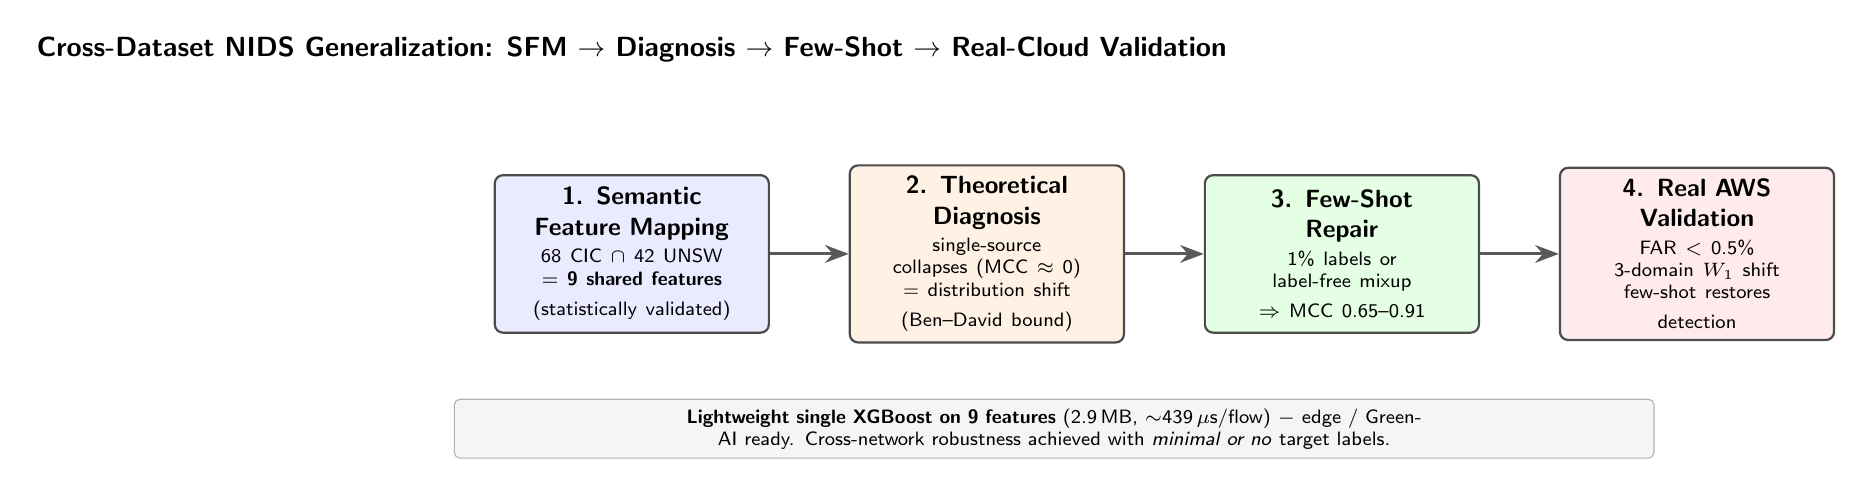
\begin{tikzpicture}[
  font=\small,
  >={Stealth[length=3mm]},
  box/.style={rounded corners=3pt, draw=black!70, line width=0.8pt,
              align=center, minimum height=20mm, text width=32mm, inner sep=4pt},
  s1/.style={box, fill=blue!8},
  s2/.style={box, fill=orange!10},
  s3/.style={box, fill=green!10},
  s4/.style={box, fill=red!8},
  lbl/.style={font=\scriptsize\bfseries, text=black!60},
  arr/.style={->, line width=1.1pt, draw=black!65},
]

% Title
\node[font=\bfseries] (title) at (0,2.6)
  {Cross-Dataset NIDS Generalization: SFM $\rightarrow$ Diagnosis $\rightarrow$ Few-Shot $\rightarrow$ Real-Cloud Validation};

% Step 1: SFM
\node[s1] (sfm) at (0,0) {\textbf{1. Semantic\\Feature Mapping}\\[2pt]
  \scriptsize 68 CIC $\cap$ 42 UNSW\\ $=$ \textbf{9 shared features}\\ (statistically validated)};

% Step 2: Diagnosis
\node[s2, right=10mm of sfm] (diag) {\textbf{2. Theoretical\\Diagnosis}\\[2pt]
  \scriptsize single-source\\ collapses (MCC $\approx$ 0)\\ = distribution shift\\ (Ben--David bound)};

% Step 3: Few-shot repair
\node[s3, right=10mm of diag] (fs) {\textbf{3. Few-Shot\\Repair}\\[2pt]
  \scriptsize 1\% labels or\\ label-free mixup\\ $\Rightarrow$ MCC 0.65--0.91};

% Step 4: AWS validation
\node[s4, right=10mm of fs] (aws) {\textbf{4. Real AWS\\Validation}\\[2pt]
  \scriptsize FAR $<$ 0.5\%\\ 3-domain $W_1$ shift\\ few-shot restores\\ detection};

% Arrows
\draw[arr] (sfm) -- (diag);
\draw[arr] (diag) -- (fs);
\draw[arr] (fs) -- (aws);

% Bottom takeaway strip
\node[draw=black!30, fill=black!4, rounded corners=2pt, text width=150mm,
      align=center, font=\scriptsize, below=7mm of diag.south east, xshift=-9mm]
  (foot)
  {\textbf{Lightweight single XGBoost on 9 features} (2.9\,MB, $\sim$439\,$\mu$s/flow)
   $-$ edge / Green-AI ready. Cross-network robustness achieved with
   \emph{minimal or no} target labels.};

\end{tikzpicture}
\end{document}
